
当协程启动时,会发生三件事:

\begin{itemize}
\item 
创建协程框架来存储协程的必要数据,这通常发生在堆上。

但允许编译器将协程帧放在堆栈上。若协程的生命周期在调用者的生命周期内,并且编译器有足够的信息来计算帧的大小,则会发生这种情况。

\item 
协程的所有参数都会复制到帧中。

注意,引用复制为引用;这并不是说他们的值复制了。所以只要协程在运行,引用形参所引用的实参必须有效。

建议是永远不要将协程参数声明为引用。否则,可能会发生带有未定义行为的致命运行时错误。

\item 
promise对象是在框架内创建的,其目的是存储协程的状态,并在协程运行时提供用于自定义的钩子。

可以将这些对象视为“协程状态控制器”(一个控制协程行为,并可用于跟踪其状态的对象)。
\end{itemize}

图15.1可视化了这个初始化过程,并显示了在协程运行时使用promise对象的哪些自定义点。

\begin{center}
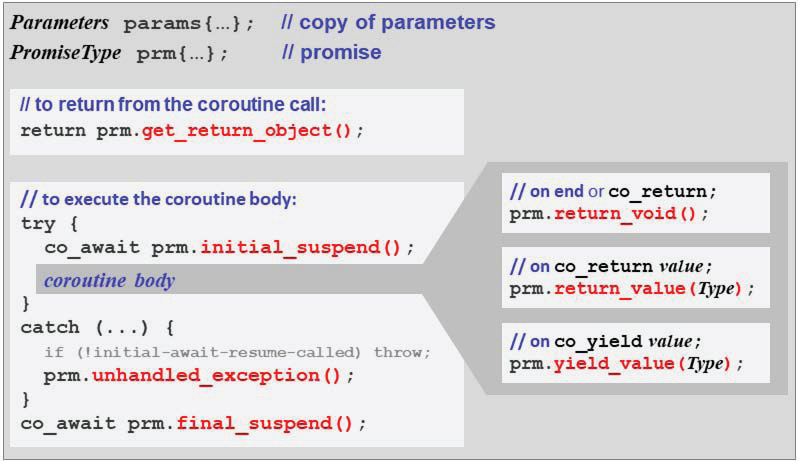
\includegraphics[width=0.8\textwidth]{content/chapter15/images/1.png}\\
图15.1 协程框架和promise
\end{center}

\mySubsubsection{15.2.1}{如何与协程接口、promise和Awaitable对象交互}

让我们再次使用awaitables,看看如何作为一个整体进行组织的:

\begin{itemize}
\item 
对于每一个启动的协程,编译器都会创建一个promise。

\item 
该promise嵌入在协程句柄中,然后放置在协程接口中,协程接口通常控制句柄及其promise的生命周期。

\item 
暂停时,协程使用awaitable对象来控制暂停和恢复时发生的事情。
\end{itemize}

下面的程序通过使用跟踪协程接口、promise和awaiter来演示精确的控制流。跟踪协程接口和promise的实现如下所示:

\filename{coro/tracingcoro.hpp}

\begin{cpp}
#include <iostream>
#include <coroutine>
#include <exception> // for terminate()

// coroutine interface to deal with a simple task
// - providing resume() to resume it
class [[nodiscard]] TracingCoro {
	public:
	// native coroutine handle and its promise type:
	struct promise_type;
	using CoroHdl = std::coroutine_handle<promise_type>;
	CoroHdl hdl; // coroutine handle
	
	// helper type for state and customization:
	struct promise_type {
		promise_type() {
			std::cout << " PROMISE: constructor\n";
		}
		~promise_type() {
			std::cout << " PROMISE: destructor\n";
		}
		auto get_return_object() { // init and return the coroutine interface
			std::cout << " PROMISE: get_return_object()\n";
			return TracingCoro{CoroHdl::from_promise(*this)};
		}
		auto initial_suspend() { // initial suspend point
			std::cout << " PROMISE: initial_suspend()\n";
			return std::suspend_always{}; // - start lazily
		}
		void unhandled_exception() { // deal with exceptions
			std::cout << " PROMISE: unhandled_exception()\n";
			std::terminate(); // - terminate the program
		}
		void return_void() { // deal with the end or co_return;
			std::cout << " PROMISE: return_void()\n";
		}
		auto final_suspend() noexcept { // final suspend point
			std::cout << " PROMISE: final_suspend()\n";
			return std::suspend_always{}; // - suspend immediately
		}
	};
	
	// constructor and destructor:
	TracingCoro(auto h)
	: hdl{h} { // store coroutine handle in interface
	std::cout << " INTERFACE: construct\n";
	}
	~TracingCoro() {
		std::cout << " INTERFACE: destruct\n";
		if (hdl) {
			hdl.destroy(); // destroy coroutine handle
		}
	}
	
	// don’t copy or move:
	TracingCoro(const TracingCoro&) = delete;
	TracingCoro& operator=(const TracingCoro&) = delete;
	
	// API to resume the coroutine
	// - returns whether there is still something to process
	bool resume() const {
		std::cout << " INTERFACE: resume()\n";
		if (!hdl || hdl.done()) {
			return false; // nothing (more) to process
		}
		hdl.resume(); // RESUME
		return !hdl.done();
	}
};
\end{cpp}

我们跟踪:

\begin{itemize}
\item 
当协程接口初始化和销毁时

\item 
当协程接口恢复协程时

\item 
每个promise操作
\end{itemize}

跟踪awaiter的实现如下:

\filename{coro/tracingawaiter.hpp}

\begin{cpp}
#include <iostream>

class TracingAwaiter {
	inline static int maxId = 0;
	int id;
	public:
	TracingAwaiter() : id{++maxId} {
		std::cout << " AWAITER" << id << ": ==> constructor\n";
	}
	~TracingAwaiter() {
		std::cout << " AWAITER" << id << ": <== destructor\n";
	}
	// don’t copy or move:
	TracingAwaiter(const TracingAwaiter&) = delete;
	TracingAwaiter& operator=(const TracingAwaiter&) = delete;
	
	// constexpr
	bool await_ready() const noexcept {
		std::cout << " AWAITER" << id << ": await_ready()\n";
		return false; // true: do NOT (try to) suspend
	}
	
	// Return type/value means:
	// - void: do suspend
	// - bool: true: do suspend
	// - handle: resume coro of the handle
	// constexpr
	bool await_suspend(auto) const noexcept {
		std::cout << " AWAITER" << id << ": await_suspend()\n";
		return false;
	}
	
	// constexpr
	void await_resume() const noexcept {
		std::cout << " AWAITER" << id << ": await_resume()\n";
	}
};
\end{cpp}

这里,我们还跟踪每个操作。

注意,成员函数不能是constexpr,因为它们有I/O。

协程的实现和使用如下所示:

\filename{coro/corotrace.cpp}

\begin{cpp}
#include "tracingcoro.hpp"
#include "tracingawaiter.hpp"
#include <iostream>

TracingCoro coro(int max)
{
	std::cout << " START coro(" << max << ")\n";
	for (int i = 1; i <= max; ++i) {
		std::cout << "  CORO: " << i << '/' << max << '\n';
		co_await TracingAwaiter{}; // SUSPEND
		std::cout << "   CONTINUE coro(" << max << ")\n";
	}
	std::cout << "  END coro(" << max << ")\n";
}

int main()
{
	// start coroutine:
	std::cout << "**** start coro()\n";
	auto coroTask = coro(3); // init coroutine
	std::cout << "**** coro() started\n";
	
	// loop to resume the coroutine until it is done:
	std::cout << "\n**** resume coro() in loop\n";
	while (coroTask.resume()) { // RESUME
		std::cout << "**** coro() suspended\n";
		...
		std::cout << "\n**** resume coro() in loop\n";
	}
	
	std::cout << "\n**** coro() loop done\n";
}
\end{cpp}

该程序有以下输出:

\begin{shell}
**** start coro()
      PROMISE: constructor
      PROMISE: get_return_object()
        INTERFACE: construct
      PROMISE: initial_suspend()
**** coro() started

**** resume coro() in loop
        INTERFACE: resume()
  START coro(3)
  CORO: 1/3
          AWAITER1: ==> constructor
          AWAITER1: await_ready()
          AWAITER1: await_suspend()
**** coro() suspended

**** resume coro() in loop
        INTERFACE: resume()
          AWAITER1: await_resume()
          AWAITER1: <== destructor
  CONTINUE coro(3)
  CORO: 2/3
          AWAITER2: ==> constructor
          AWAITER2: await_ready()
          AWAITER2: await_suspend()
**** coro() suspended

**** resume coro() in loop
        INTERFACE: resume()
          AWAITER2: await_resume()
          AWAITER2: <== destructor
  CONTINUE coro(3)
  CORO: 3/3
          AWAITER3: ==> constructor
          AWAITER3: await_ready()
          AWAITER3: await_suspend()
**** coro() suspended

**** resume coro() in loop
        INTERFACE: resume()
          AWAITER3: await_resume()
          AWAITER3: <== destructor
  CONTINUE coro(3)
  END coro(3)
      PROMISE: return_void()
      PROMISE: final_suspend()
      
**** coro() loop done
        INTERFACE: destruct
      PROMISE: destructor
\end{shell}

当调用协程时,发生的第一件事就是创建协程的promise。

然后,对创建的promise调用get\_return\_object()方法,这个函数通常初始化协程句柄并返回用它初始化的协程接口。要创建句柄,通常会调用from\_promise()中的静态成员函数,然后传递句柄来初始化TracingCoro类型的协程接口,再将协程接口返回给get\_return\_object()的调用者,以便它可以用作协程调用的返回值(极少数情况下可能有其他返回类型)。

然后,调用initial\_suspend()来查看是否应该立即挂起协程(惰性启动),所以控制流会返回给协程的调用者。

稍后,main()调用resume(),resume()为协程句柄调用resume()。此调用恢复协程,所以协程将处理以下语句,直到下一次挂起或结束。

对于每个暂停,co\_await都会使用一个awaitable对象,在本例中它是一个类型为TracingAwaiter的awaiter对象,是用默认构造函数创建的。对于awaiter,调用成员函数await\_ready()和await\_suspend()来控制挂起(甚至可能拒绝挂起)。因为await\_ready()返回false,而await\_suspend()不返回任何值,所以接受挂起请求。因此,协程的恢复结束,main()继续。下一次恢复时,调用await\_resume()并继续协程。

当协程到达其结束或co\_return语句时,将调用处理其结束的相应成员函数。首先,根据是否有返回值,调用return\_void()或return\_value()。然后,调用用于最终挂起的函数final\_suspend()。注意,即使在final\_suspend()中,协程仍在“运行”,则再次调用resume(),或在final\_suspend()中调用destroy(),将导致运行时错误。

在协程接口生命周期结束时,调用其析构函数,析构函数将销毁协程句柄。最后,销毁promise。

作为一种替代方案,假设初始化的\_suspend()返回一个promise类型,表示提前启动协程,而不是一开始挂起它:

\begin{cpp}
class [[nodiscard]] TracingCoro {
	public:
	...
	struct promise_type {
		...
		auto initial_suspend() { // initial suspend point
			std::cout << " PROMISE: initial_suspend()\n";
			return std::suspend_never{}; // - start eagerly
		}
		...
	};
	...
};
\end{cpp}

将得到以下输出:

\begin{shell}
**** start coro()
      PROMISE: constructor
      PROMISE: get_return_object()
        INTERFACE: construct
      PROMISE: initial_suspend()
  START coro(3)
  CORO: 1/3
          AWAITER1: ==> constructor
          AWAITER1: await_ready()
          AWAITER1: await_suspend()
**** coro() started

**** resume coro() in loop
        INTERFACE: resume()
          AWAITER1: await_resume()
          AWAITER1: <== destructor
  CONTINUE coro(3)
  CORO: 2/3
          AWAITER2: ==> constructor
          AWAITER2: await_ready()
          AWAITER2: await_suspend()
**** coro() suspended

**** resume coro() in loop
        INTERFACE: resume()
          AWAITER2: await_resume()
          AWAITER2: <== destructor
  CONTINUE coro(3)
  CORO: 3/3
          AWAITER3: ==> constructor
          AWAITER3: await_ready()
          AWAITER3: await_suspend()
**** coro() suspended

**** resume coro() in loop
        INTERFACE: resume()
          AWAITER3: await_resume()
          AWAITER3: <== destructor
  CONTINUE coro(3)
  END coro(3)
      PROMISE: return_void()
      PROMISE: final_suspend()
      
**** coro() loop done
        INTERFACE: destruct
      PROMISE: destructor
\end{shell}

同样,协程框架创建了promise,并对其调用get\_return\_object(),这初始化了协程句柄和协程接口,但initial\_suspend()不会挂起。因此,协程开始急切地执行第一个语句,直到第一个co\_await第一次挂起。当最初在get\_return\_object()中创建的TracingCoro对象返回给协程的调用者时,就触发了这个暂停。之后,和前面一样,恢复循环遍历。









